% !TEX root = ../thesis-example.tex
%
\chapter{Patterns of segregation}
\label{chap:patterns_segregation}

\begin{flushright}{\slshape    
To understand is to perceive patterns.} \\ \medskip
--- Isaiah Berlin~\cite{Berlin:2013}
\end{flushright}


\bigskip


\section{Introduction}
\label{sec:introduction}

\subsection{Shortcomings in the current empirical picture}
\label{sub:shortcomings_in_the_current_empirical_picture}

There are many different ways in which a spatial pattern can deviate from its
randomised counterpart, and at least as many different measures one could
perform. In this chapter, we will try to quantify these patterns in a way that
may allow us to \emph{understand} the phenomenon of segregation.\\

Of course, segregation has been extensively studied in the literature. However,
we identify several difficulties in the current empirical picture.

First, some issues are tied to the existence of several categories in the
underlying data. Historically, measurements of racial segregation were limited
to measures between $2$ population groups. However, most measures generalise
poorly to a situation with many groups, and the others do not necessarily have a
clear interpretation~\cite{Reardon:2002}. Worse, in the case of groups based on
a continuum (such as income), the thresholds chosen to define classes are
usually arbitrary~\cite{Jargowsky:1996}. We propose to solve this issue by
defining classes in a unambiguous and non-arbitrary way through their pattern of
spatial interaction. Applied to the distribution of income categories in US
cities, we find $3$ emergent categories, which are naturally intepreted as the
lower-, middle- and higher-income classes.

Second, most authors systematically design a single index of segregation for
territories that can be very large, up to thousands of square
kilometers~\cite{Apparicio:2000}. In order to mitigate segregation, a more
local, spatial information is however needed: local authorities need to locate
where the poorest and richest concentrate if they want to design efficient
policies to curb, or compensate for, the existing segregation. Furthermore, 
a local description of the repartition of the different categories is the first
step towards the exploration of the mechanisms responsible for segregation: it
is necessary to gather hints (as well as empirical regularities) that are
essential to build a reasonable model. 
In other words, we need to provide a clear {\it spatial} information on the
pattern of segregation.\\



The lack of clear spatial characterization of the distribution of individuals is
not tied to the problem of segregation in particular, but pertains to the field
of spatial statistics~\cite{Ripley:1981}. Many studies avoided this spatial
problem by considering cities as monocentric and circular, and rely on either an
arbitrary definition of the city center boundaries, or on indices computed as a
function to the distance to the center (whatever this center may be, see
Part~\ref{part:polycentricity}). However, most if
not all cities are anistropic, and the large ones, polycentric
(see Chapter~\ref{chap:monocentric_introduction}), casting some doubt about
the application of the monocentric city picture. Many empirical studies and
models in economics aim to explain the difference between central cities and
suburbs \cite{Glaeser:2008, Brueckner:1999}. Yet, the sole stylized fact upon
which they rely -- city centers tend are allegedly poorer than suburbs (in the US) --
lacks a solid empirical basis.\\

In the following, we propose to answer the following questions

\begin{itemize}
    \item How can we quantify the presence of the different categories in areal
        units? Can we say whether they are overrepresented or normally
        represented? How can we define neighbourhoods?
    \item Can we quantify interactions between the different categories?
    \item Can we define meaningful classes from the original data?
    \item Do classes tend to leave in geographically coherent areas, or are they
        scattered across the city?
    \item Is there a difference between the city center and the suburbs? How
        can we quantify this adequately?
\end{itemize}

\subsection{Notations}
\label{sub:notations}

In the following, we will illustrate our measures using data from the $2000$ US
Census on the income of households per Census blockgroup. Data present
themselves as a number of households per blockgroup, sorted in different income
categories. There are $N$ individuals and  $T$ tracts in the considered
geographical area, and we note $N_\alpha$ the number of individuals belonging to
the category $\alpha$.  Finally, we write $n(t)$ the total number of individuals
living in the tract $t$, and $n_\alpha(t)$ the total number of individuals who
belong to category $\alpha$ living in the tract $t$.



\section{Presence of categories}
\label{sec:presence_of_categories}

In order to quantify segregation, we first need to measure the extent to which
categories are spread unevenly across space. Therefore, we start our analysis
with a discussion on how to quantify the presence of a category in areal units.
Several indicators exist, and one needs to be aware of their meaning, their
qualities and their shortcomings. 


\subsection{Concentration index}
\label{sub:concentration}

The concentration index measures the proportion of individuals from category $\alpha$
in the areal unit $t$. 

\begin{equation}
    c(t) = \frac{n_\alpha(t)}{N_\alpha}
    \label{eq:concentration}
\end{equation}

The concentration is composition-invariant: it
does not depend on the relative proportion of category $\alpha$ in the
geographical zone as a whole. 

Nevertheless, its value strongly depends on the total population of the areal
unit we are studying: more populated areal units mechanically entail higher
values of concentration. Segregation measures based on the concentration
(such as the dissimilarity index) will therefore be dominated by the values in
highly populated areal units. This also makes values of concentration difficult
to intepret: we don't know whether large (repectively low) values of
concentration are the result of a large (respective low) population, or of a
local concentration of individuals in the area. 


\subsection{Proportion index}
\label{sub:proportion}

Sometimes, we would prefer to know the proportion of individuals of a given
category in a unit. In our notations, the proportion index is simply defined as 

\begin{equation}
    p(t) = \frac{n_\alpha(t)}{n(t)}
\end{equation}

Although the values of the proportion index are easier to interpret (``x\% of the
individuals living in this areal unit belong to such category''), they are
not a good indicator of segregation. 

Indeed, they strongly depend on the relative proportion of individuals of the
category in the geographical area being studied. For instance, in a city where
$90\%$ of the individuals belong to category $A$, the proportion of people
belonging to category $A$ is very likely to be high in all areal units in the city.
The measure of proportion is therefore strongly tied to the overall inequality
levels.


\subsection{An unbiaised measure: representation}
\label{sub:an_unbiaised_measure_the_representation}

\subsubsection{Definition}
\label{ssub:definition}

The representation solves the problems linked to both measures of concentration
and proportion. The idea behind the measure of representation is that
segregation is, as we argued in Chapter~\ref{chap:segregation_introduction}, a
departure from the situation where households would be spatially distributed
at random. The properties of such a `random', unsegregated city are well known,
and the distribution of categories in each areal unit is given by a binomial
distribution. The representation is
thus defined as the number $n_\alpha(t)$ divided by its expected value in an
unsegregated city, $N_\alpha\,\frac{n(t)}{N}$

\begin{equation}
    r_\alpha(t) = \frac{n_\alpha(t)/n(t)}{N_\alpha/N}
    \label{eq:representation}
\end{equation}

Another way to understand the representation is to compare it to the
above-defined concentration and proportion. We can indeed write

\begin{equation}
    r_\alpha(t) = \frac{c(t)}{n(t) / N} = \frac{p(t)}{N_\alpha/N}
\end{equation}

The representation can thus be interpreted as the concentration
normalised by the local population concentration, or the proportion renormalised
by the proportion of the category at the city level, thereby addressing the
aforementioned shortcomings.\\


\subsubsection{Measuring significant deviations}
\label{ssub:measuring_significant_deviations}


The representation $r_\alpha(t)$ takes values between $0$ (when no
individuals from the category $\alpha$ are present in $t$) and
$\frac{N}{N_\alpha}$ (when all individuals in $t$ belong to the category
$\alpha$). In a city where individuals are distributed uniformly
(see Chapter~\ref{chap:segregation_introduction}), $r_\alpha(t) = 1$ in every
tract $t$.\\


In an unsegregated situation, the values of the representation are likely to be
close to $1$, but not necessarily strictly equal to $1$. There is indeed a
non-zero probability for any distribution to be obtained by chance. It is
therefore not obvious whether a given value of representation could have been
obtained in the unsegregated configuration. However, to quantify segregation, we
need to know how \emph{likely} it is that the present pattern is not the result
of a random repartition of individuals.  In other words, we need to know
whether areal units depart \emph{significantly} from the unsegregated situation. 

The distribution of individuals in a tract $t$ in the unsegregated city follows
a binomial distribution. We can therefore easily compute how likely it is that
the representation $r_\alpha(t)$ we measure has been obtained by chance. To do
that, we first compute the variance of the representation in the unsegregated
configuration:

\begin{equation}
    \mathrm{Var}\left[r_\alpha(t)\right] = \sigma_\alpha(t)^2 = \frac{1}{N_\alpha} \left[\frac{N}{n(t)} - 1\right]
\end{equation}

We say that the representation departs \emph{significantly} from the
unsegregated configuration if we can be sure with $99\%$ confidence that the
pattern has not been obtained at random. It follows that

\begin{itemize}
    \item $\alpha$ is {\bf overrepresented} in $t$ iff $r_\alpha(t) > 1 +
  2.57\;\sigma_\alpha(t)$
    \item $\alpha$ is {\bf underrepresented} in $t$ iff $r_\alpha(t) < 1 +
  2.57\;\sigma_\alpha(t)$
\end{itemize}

Note that the expression of the representation (Eq. \ref{eq:representation}) is very
similar to the formula used in economics to compute comparative
advantages~\cite{Balassa:1965}, or to the localisation quotient used in various
contexts~\cite{Apparicio:2000, Schwabe:2011}. To our knowledge, however, this
formula has never been justified by a null model in the context of residential
location. 

The representation allows to assess the significance of the deviation
of population distributions from the unsegregated city. As we will show below,
it is also the building block for measuring the level of repulsion or attraction
between populations -- allowing us to uncover the different classes -- and to
identify the neighbourhoods where the different categories concentrate. 

Last, but not least, the representation defined here does not depend on the
class structure at the city scale, but only on the spatial repartition of
individuals belonging to each class. This is essential to be able to compare
different cities where the group compositions -- or inequality -- might differ.
Inequality and segregation are indeed two separate concepts, and the way they
are measured should be distinct from one another. In that sense, the
representation is preferable to the measures of concentration or representation
as a basis to quantify segregation.


\section{Measuring the attraction and repulsion of categories}
\label{sec:measuring_the_attraction_and_repulsion_of_categories}

\subsection{Exposure}
\label{sub:exposure}

If we want to uncover the mechanisms underlying segregated patterns, it is
important to measure and understand the interactions between categories.
However, existing measures do not allow to quantify to which extent different populations
attract or repel one another. What we mean here by interaction is the
co-presence of the different categories in the same areal units, thus potential
interactions. This is the best one can do in the absence of data on the actual
interactions between individuals.

The measure we define is inspired by the M-value first introduced by Marcon \&
Puech in the economics literature~\cite{Marcon:2009} and used as a measure of
interaction in \cite{Jensen:2006}.  These authors were interested in measuring
the geographic concentration of different types of industries. While previous
measures (such as Ripley's K-value) allow to identify departures from a random
(Poisson) distribution, the M-value's interest resides in the possibility to
evaluate different industries' tendency to co-locate.\\

The idea, in the context of segregation, is simple. We consider two categories
$\alpha$ and $\beta$ and we would like to measure to which extent they are
co-located in the same areal unit. Essentially, we measure the representation of
the category $\beta$ as witnessed on average by the individuals in category
$\alpha$, and obtain the following quantity $E_{\alpha\beta}$

\begin{equation} 
    E_{\alpha \beta} = \frac{1}{N_\alpha} \sum_{t=1}^{T} n_\alpha(t)\,r_\beta(t) 
\end{equation}

Although it is not obvious with this formulation, this measure is symmetric:
$E_{\alpha \beta} = E_{\beta \alpha}$. Effectively, the E-value is a measure of exposure,
according to the typology of segregation measures found in~\cite{Massey:1988}.
It is however different from the traditional measure of exposure found in the
literature~\cite{Bell:1954}, as it allows to distinguish between the situations
where categories attract, or repel one another.\\

In the case of an unsegregated city, every household in $\alpha$ sees
on average $r_\beta = 1$ and we have $E_{\alpha \beta} = 1$. 
If populations $\alpha$ and $\beta$ {\em attract} one another, that is if they
tend to be overrepresented in the same areal units, every household $\alpha$
sees $r_\beta > 1$ and we have $E_{\alpha \beta} > 1$ at the city scale. 
On the other hand, if they
{\em repel} one another, every household $\alpha$ sees $r_\beta < 1$
and we have $E_{\alpha \beta} <1$ at the city scale. 


\subsection{Extreme values}
\label{sub:extreme_values}

The minimum of the exposure for two classes $\alpha$ and $\beta$ is obtained
when these two categories are never present together in the same areal unit. Then

\begin{equation}
    E_{\alpha\,\beta}^{min} = 0 
\end{equation}

and the theoretical maximum is obtained when the two classes are alone in the system and
otherwise distributed at random

\begin{equation}
    E_{\alpha\,\beta}^{max} = \frac{N^2}{4\,N_\alpha\, N_\beta}
\end{equation}

These extrema are useful when comparing the exposure values for different
categories, and across different cities.



\subsection{Isolation}
\label{sub:isolation}

In the case $\alpha = \beta$, the previous measure represents the
`isolation' defined as

\begin{equation}
    I_\alpha = \frac{1}{N_\alpha}\sum_{t=1}^{t} n_\alpha(t)\,r_\alpha(t)
\end{equation}

and measures to which extent individuals from the same category are
exposed to their kins. In the unsegregated city, where individuals are
indifferent to others when choosing their residence, we have
$I_\alpha^{min}=1$. On the other hand, in the extreme situation where
individuals belonging to the class $\alpha$ live isolated from the
others, the isolation reaches its maximum value

\begin{equation}
    I_\alpha^{max} = \frac{N}{N_\alpha}
\end{equation}

%Of course, in order to discuss the significance of the values of exposure and
%isolation, one needs to compute the variance of the exposure in the unsegregated
%situation defined earlier. The calculations for the variance as well as for the
%extrema are presented in the Supporting Information. [WATCH FOR THIS ONE]

\section{Emergent social classes}
\label{sec:the_emergent_social_classes}

\subsection{Defining classes}
\label{sub:defining_classes}


The study of income segregation must be rooted in a particular definition of categories
(or classes). There is however no consensus in the literature about how to
separate households in different classes according to their income, and studies
generally rely on more or less arbitrary divisions. While in some particular
cases grouping the original categories in pre-defined classes is justified,
most authors do so for mere convenience. However, as some sociologists
have already pointed out~\cite{Emirbayer:1997}, imposing the existence of
absolute, artificial entities is necessarily going to skew our reading of the
data. Entities such as social classes do not have an existence of their own.
Grouping the individuals into arbitrary classes when studying segregation is
thus problematic: it amounts to imposing a class structure on the society before
assessing the existence of this structure (which manifests itself by the
differentiated spatial repartition of individuals with different income,
segregation).
Furthermore, in the absence of recognized standards, different authors will
likely have different definitions of classes, making the comparisons between
different results in the literature difficult.\\

Here, instead of imposing an arbitrary class structure , we let the class
structure emerge from the data themselves. Our starting hypothesis is the
following: if there is such a thing as a social stratification based on income,
it should be reflected in the households' behaviours. The hypothesis is that households belonging to
the same class should tend to live together, while households belonging to
different classes should tend to avoid one another (It is worth noting that this
\emph{horizontal} definition of segregation is not relevant in every context; in
the 19th century Paris for instance, segregation was also vertical, with rich families
living in the lowest floors of buildings while poor individuals did tend to
live in the highest flats). The idea is thus to define
classes based on the way they manifest themselves through the spatial
repartition of the different categories. Of course, spatial proximity does not
necessarily imply social proximity. In particular, Chamboredon showed that in
some big French housing projects, households belonging to different social
classes were artificially brought in close proximity to one another but did not
necessarily interact with one another~\cite{Chamboredon:1970}\graffito{The work of
Chamboredon was kindly brought to my attention by Yann Renisio.}. We thus assume
here that the social class of housing tenants is not determined in a top-down
fashion, so that the spatial repartition of different income classes reflects
the nature of the interaction between these classes. 


\subsection{Income classes in the US}
\label{sub:income_classes_in_the_u_s_}

We choose as a starting point the finest income subdivision given by the Census
Bureau ($16$ subdivisions) and compute the $16 \times 16$ matrix of $E_{\alpha
\beta}$ values for all cities. We then perform a hierarchical clustering on this
matrix, successively aggregating the subdivisions with the highest $E_{\alpha
\beta}$ values. We stop the aggregation process when the only classes left are
indifferent ($E_{\alpha \beta} = 1$ with $99\%$ confidence) or
repel one another ($E_{\alpha \beta} < 1$ with $99\%$
confidence)~\cite{Louf:2015}. We obtain the dendrogram presented on
Figure~\ref{fig:classes_alluvial}.

\begin{figure}
    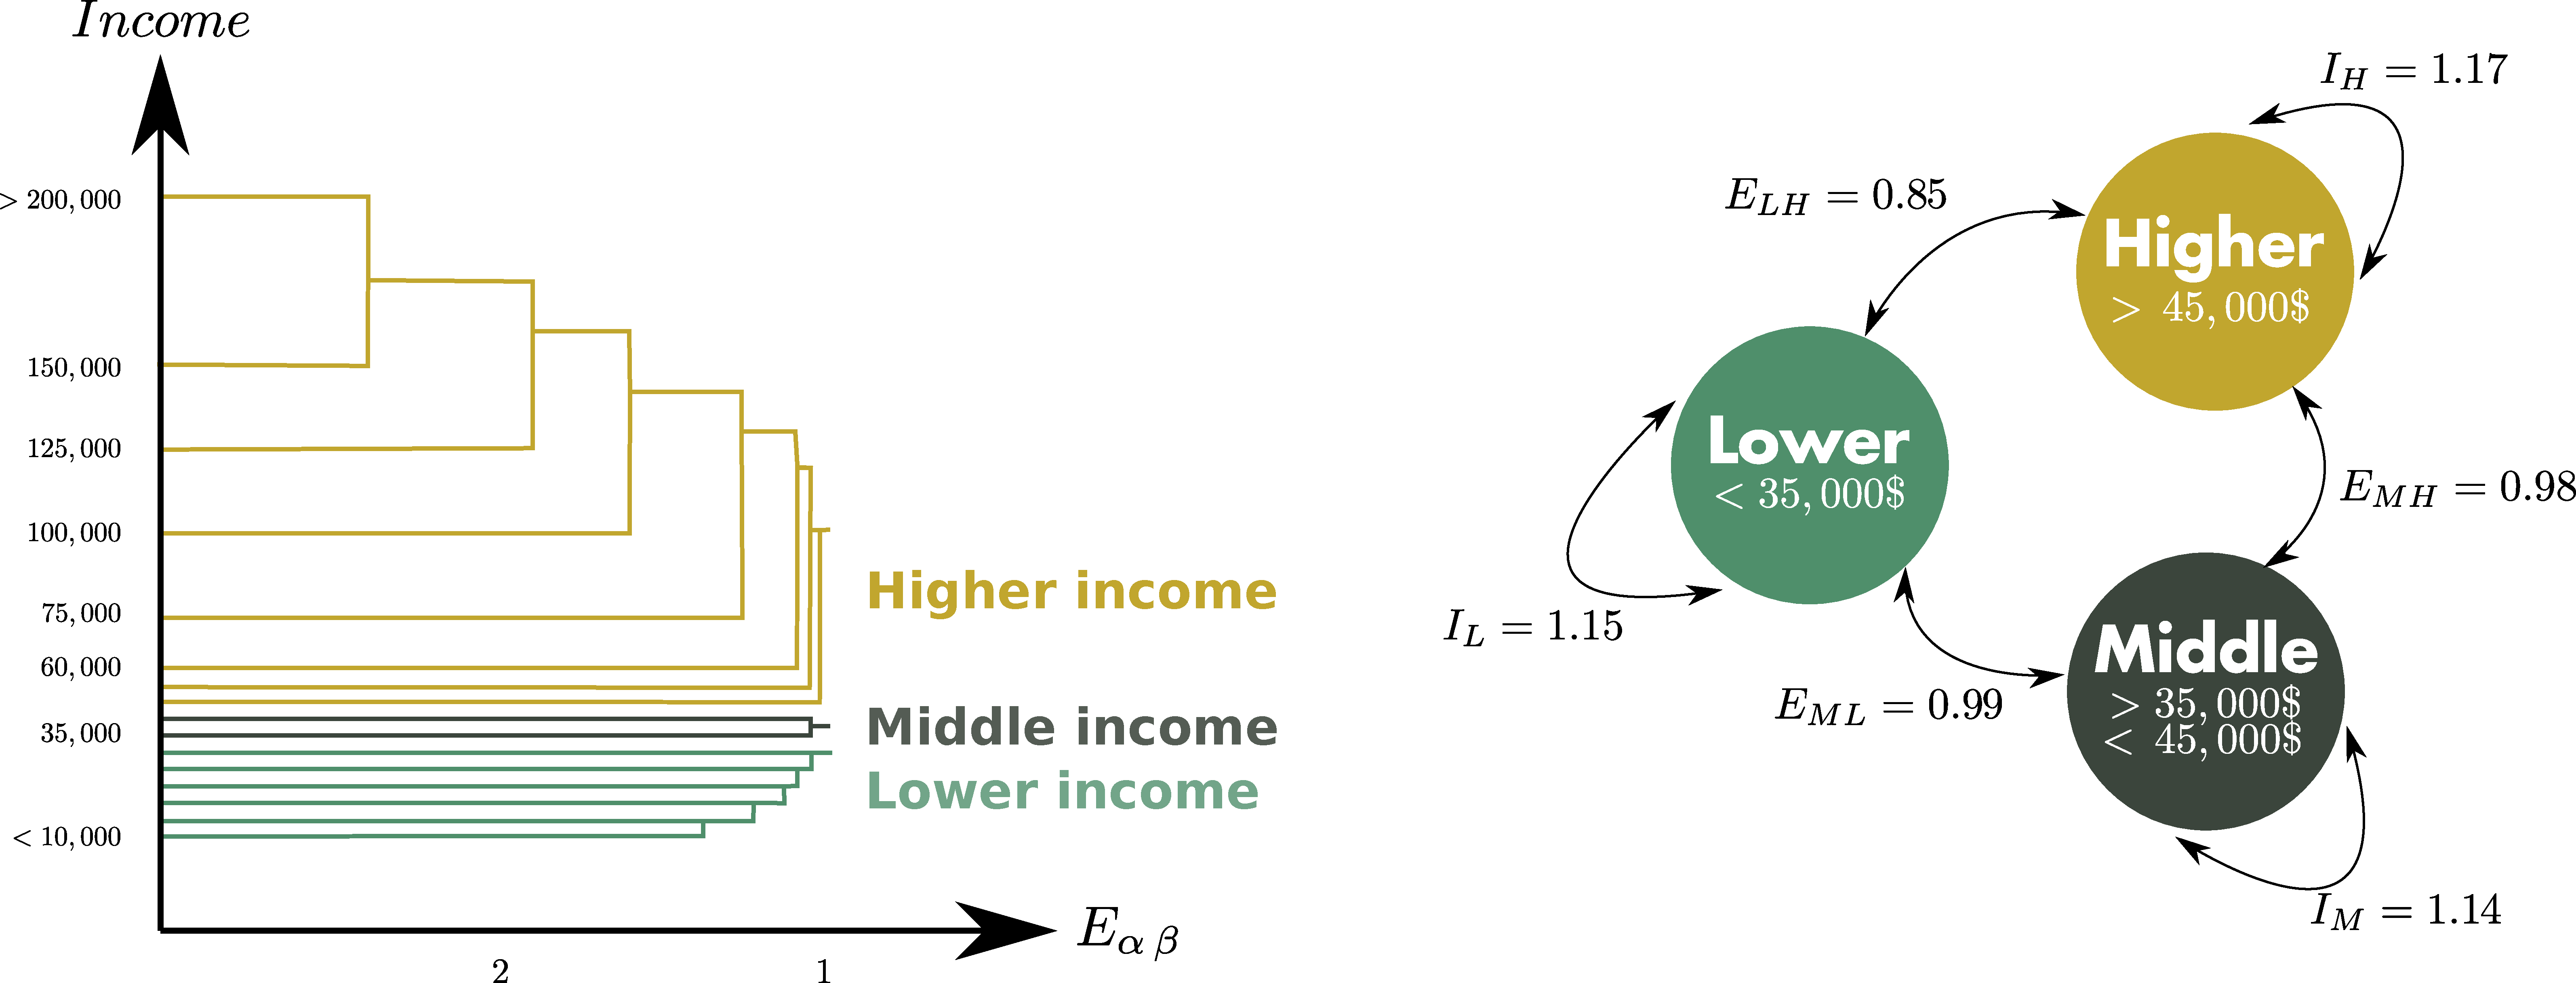
\includegraphics[width=\textwidth]{./gfx/chapter-segregation/figure1.pdf}
    \caption{{\bf Emergent classes.} (Left) Alluvial diagram showing the successive aggregations
      of income categories in the clustering process, and
      the value of the exposure at which the aggregation took
      place. The aggregation stops when there is no pair of category
      for which $E>1$, that is when all classes are at best
      indifferent to one another. One can see on this diagram that
      the highest income categories attract one another more (higher values of
      $E_{\alpha \beta}$) than the lowest income categories. (Right) The classes that emerge from our
      analysis, and their respective exposure and isolation values. The lower
      and higher income classes repel one another, while the middle
      income class is indifferent to either other classes.  The
      higher-income class is slightly more coherent than the lower-income,
      which is more coherent than the middle-income class, as
      reflected by the isolation coefficient $I$.}
\label{fig:classes_alluvial}
\end{figure}

Strikingly, the outcome of this method is the emergence of 3 distinct classes:
the higher-income ($47\%$ of the US population) and the lower-income ($42\%$ of the US population) classes
 -- which repel one another strongly while being
respectively very coherent -- and a somewhat meagre middle-income class ($11\%$
of the population) that is relatively indifferent to the other classes. This
result implies that there is some truth in the conventional way of dividing
populations into $3$ income classes, and that what we casually perceive as the
social stratification in our cities actually emerges from the spatial
interaction of people. Surprisingly, however, the middle-income class as
obtained here represents a significantly smaller part of the population than
other definitions.

Our method has several advantages over a casual, arbitrary definition: it only
depends on single tunable parameter, the size of the confidence interval.
Although, once an agreement has been reached, the class structure does not
depend on who is performing the analysis. Its origins are tractable, and can be argued on a
quantitative basis. Because it is quantitative, it allows comparison of the
stratification between different points in time, or between different countries. It
can also be compared to other class divisions that would be obtained using a
different medium for interaction, for instance mobile phone
communications~\cite{Eagle:2010}. 

In the following, we will systematically use the classes thus obtained.



\section{Larger cities are richer}
\label{sec:inter_urban}

At the scale of an entire country, segregation can manifest itself in the
unequal representation of the income classes in different urban areas.
We plot on Figure~\ref{fig:inter-urban} the ratio $
N_\alpha^{>}(H)/N^{>}(H)$ where $N^{>}(H)$ is the number of cities of
population greater than $H$, and $N_\alpha^{>}(H)$ the number of cities of
population greater than $H$ for which the class $\alpha$ is overrepresented.

\begin{figure}[!h]
    \centering
    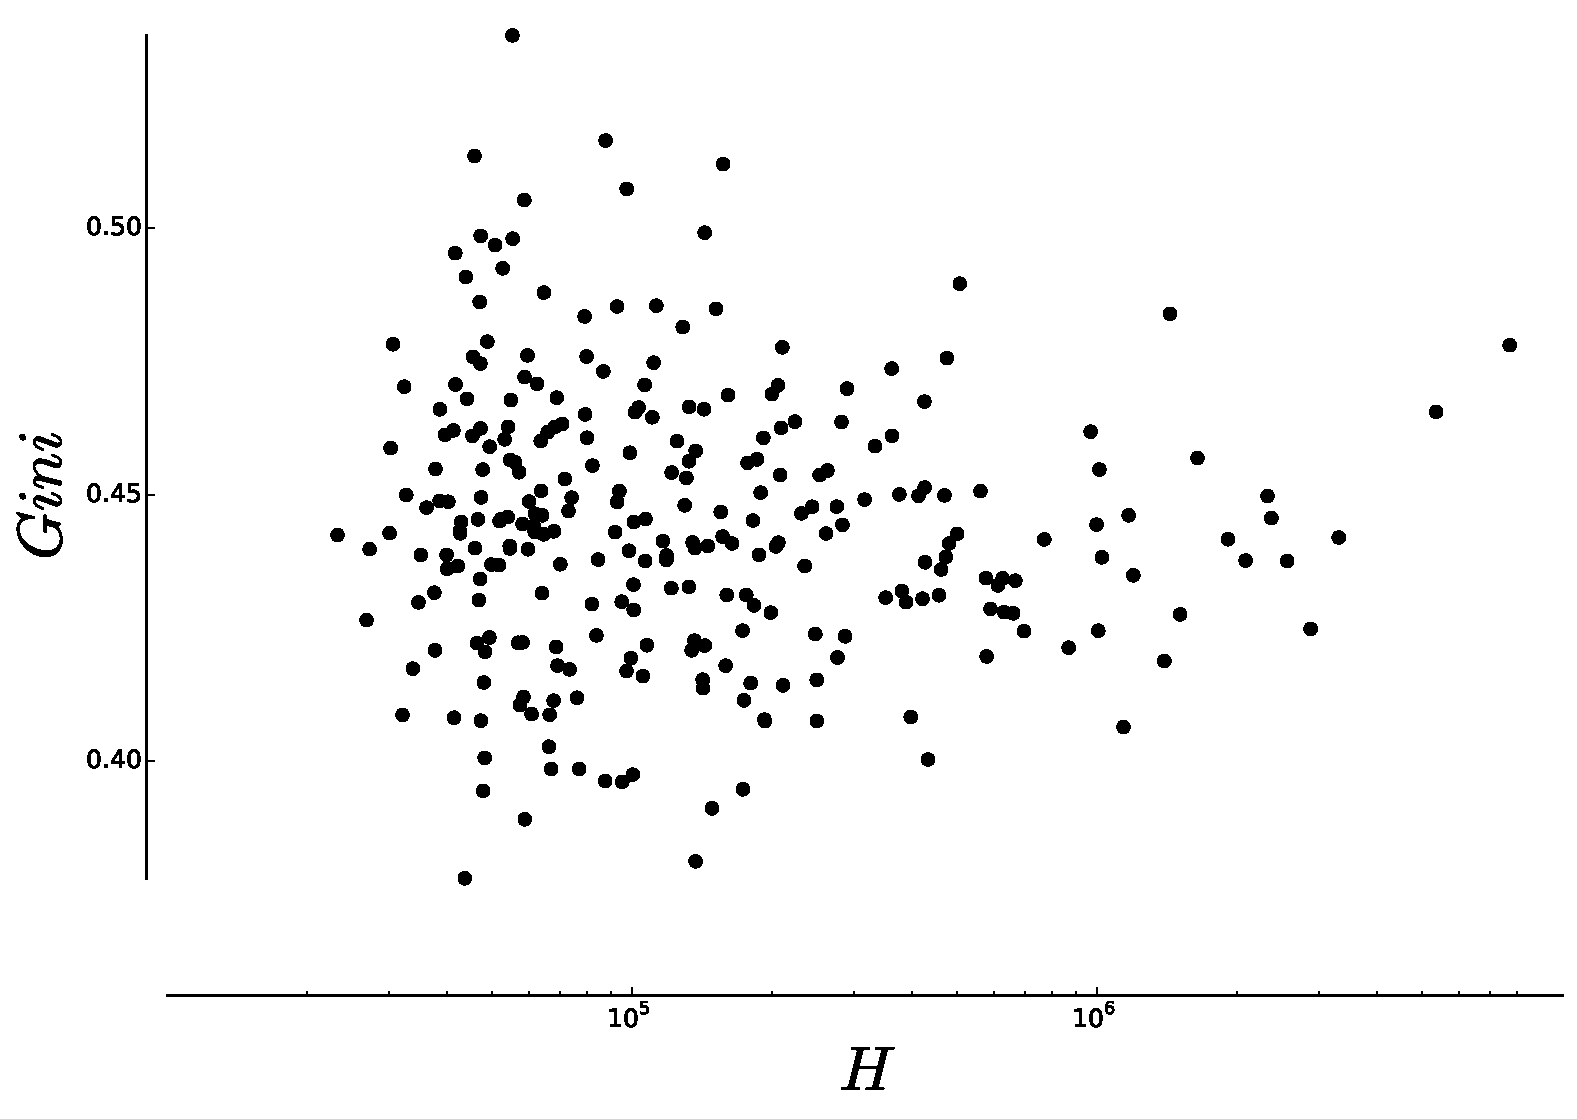
\includegraphics[width=0.7\textwidth]{./gfx/chapter-segregation/gini_income.pdf}
    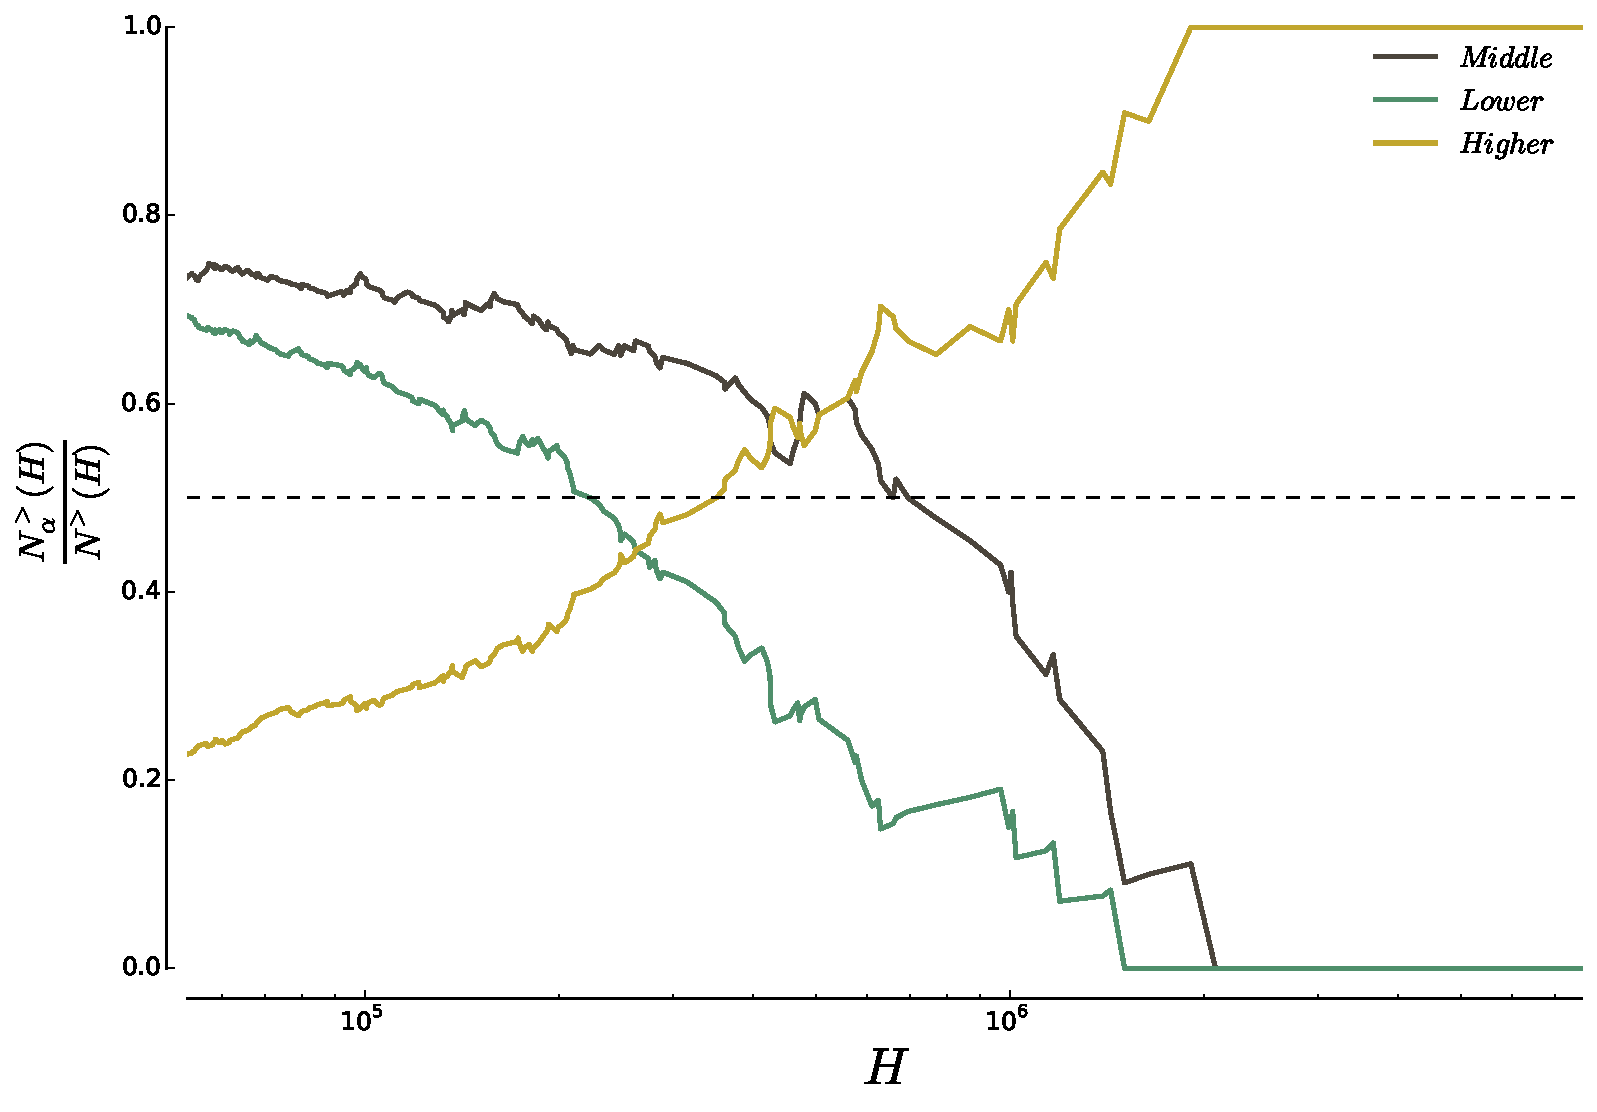
\includegraphics[width=0.7\textwidth]{gfx/chapter-segregation/figure3.pdf}
    \caption{{\bf Larger cities are richer.} (Top) Gini coefficient of the income distribution of the $280$ MSA in
    $2000$ versus the number of households in the city. As one can see, there is
    no clear trend. (Bottom) Proportion of cities in which the different classes are
    overrepresented, as a function of the total population of the city. One can
    clearly see that as cities get larger rich people will
    be overrepresented and poor people underrepresented (compared to national
    levels). \label{fig:inter-urban}}
\end{figure}

A decreasing curve indicates that the category $\alpha$ tends to be
underrepresented in larger urban areas, while an increasing curve shows that the
category $\alpha$ tends to be overrepresented in larger urban areas.  The
representation is measured with respect to the total population at the US level.

There is a clear differentiation between cities: among the $276$ MSA in our
dataset, no city exhibits a number of households per class 
that is representative of the US as a whole. Furthermore, the number of cities
where higher-income households are overrepresented increases with the size of
the cities, while the inverse trend is true for lower-income
households. Therefore, larger cities are not richer in the sense that rich
households tend to be overrepresented in large cities, and underrepresented in
small ones.

Surprisingly, this effect is not visible using the Gini coefficient (see
Figure~\ref{fig:inter-urban}). This hints at the limitations of the Gini index
to compare income inequalities across an entire country.


\section{Delineating neighbourhoods}
\label{sec:neighbourhoods}

\subsection{Defining neighbourhoods}
\label{sub:defining_neighbourhoods}

\begin{figure}
    \centering
    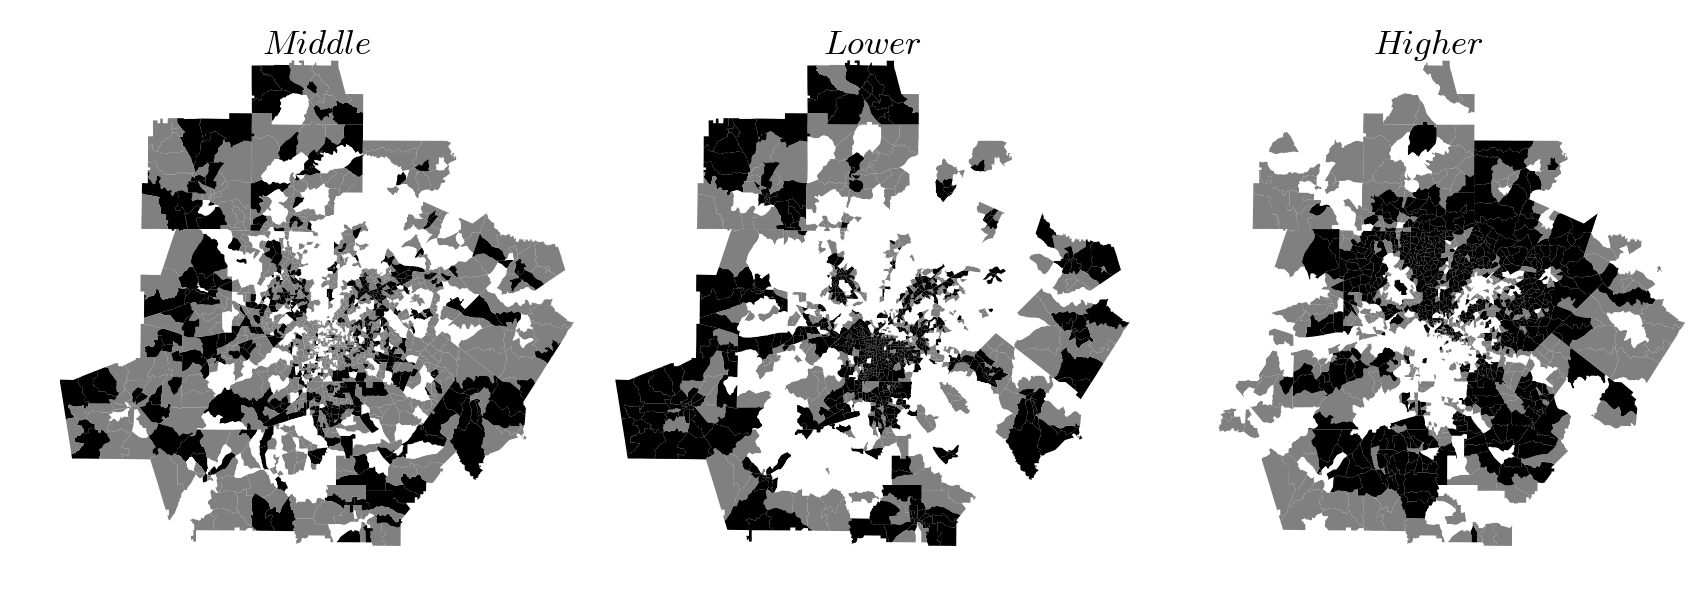
\includegraphics[width=0.7\textwidth]{./gfx/chapter-segregation/figure2.png}
    \caption{{\bf Neighbourhoods.} The neighbourhoods in Atlanta for the three different
      income category. In black, the tracts where the corresponding
      class is overrepresented, in white where it is
      underrepresented and in grey where its value is
      indistinguishable from the random distribution. All
      MSA defined for the $2000$ Census exhibit a total exclusion between
      lower-income and higher-income
      neighbourhoods: the pictures for lower- and higher-income classes are the
      perfect negative of one another. In contrast, middle-income households
      are scattered across the city.}
\label{fig:atlanta_neighbourhoods}
\end{figure}

Now that we can identify the areal units where classes are overrepresented, how
can we delineate neighbourhoods?

Considering a category $\alpha$,  we first look for the areal units where the
category is overrepresented. We then consider that two areal units in this set
are part of the same neighbourhood if they are contiguous. Of course, this
approach has limitations (some remarks that sprung in the discussion on the different methods to find
activity centers in Chapter~\ref{chap:monocentric_introduction} are relevant in
this context too), but it gives us a reasonable definition of neighbourhoods to
work with.
Let us now focus on the properties of these neighbourhoods.

\subsection{Clustering}
\label{sub:clustering}

Intra-tract measures such as the exposure are not enough to quantify
segregation. Indeed, areal units where a given class is overrepresented can
arrange themselves in different ways, without the intra-tract measures of
segregation being affected~\cite{White:1983}. In order to illustrate this, we
consider the schematic cases represented on Figure~\ref{fig:checkerboard}, and
assume that  they are obtained by reshuffling the various squares around.
Obviously, the checkerboard on the left depicts a very different segregation
situation from the divided situation on the right while intra-tract measures
would give identical results.\\

\begin{figure}[!h]
    \centering
    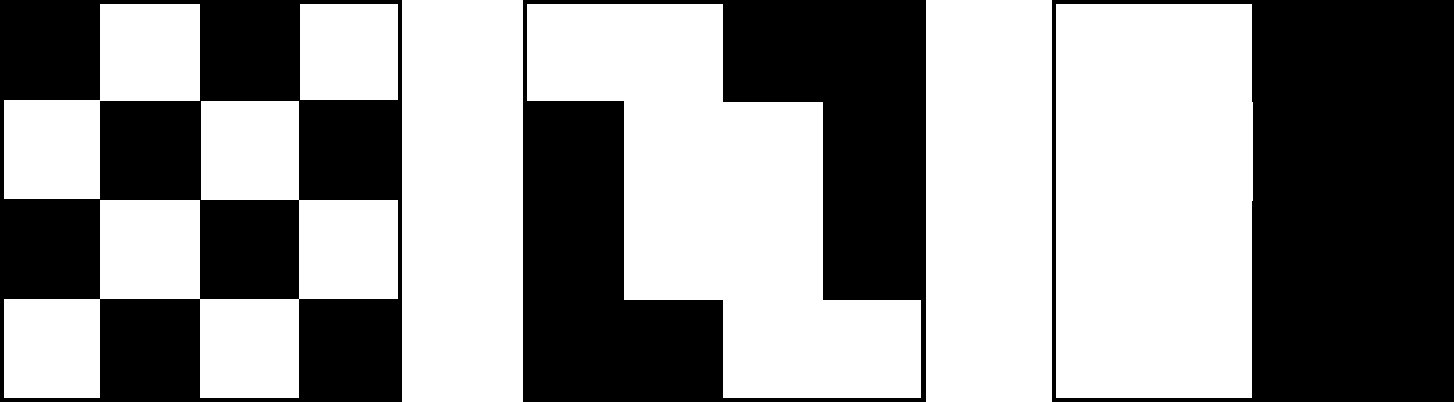
\includegraphics[width=0.7\textwidth]{./gfx/chapter-segregation/figure5.pdf}
    \caption{{\bf Spatial considerations.} Three situations that are identical for intra-areal unit measures,
        but that represent different segregation levels. (Left) The checkerboard
        city popularised by White~\cite{White:1983}, corresponding to a
        clustering value (defined in Eq.~\ref{eq:clustering}) of $C=0$ for the black squares. (Middle) An
        intermediate situation between the checkerboard and the divided city,
        corresponding to $C \approx 0.86$.(Right) The divided city, corresponding to
        $C=1$. \label{fig:checkerboard}} 
\end{figure}


A way to distinguish between different spatial arrangements is then to measure
how clustered the overrepresented areal units are. We first aggregate adjacent
overrepresented areal units (for a given class) leading to consistent
neighbourhoods. The ratio of the number $N_n$ of neighborhoods (clusters) to the
total number $N_o$ of overrepresented areal units measures the level of
clustering and in 

\begin{equation} 
    C = \frac{N_{o}-N_{n}}{N_{o}-1}
    \label{eq:clustering}
\end{equation}


such that this quantity is $C = 0$ in a checkerboard-like situation, and $C = 1$
when all areal units form a unique neighbourhood. We show on
Figure~\ref{fig:clustering} the distibution of $C$ for the three classes over all
cities in our dataset. As one could infer from the maps on
Figure~\ref{fig:atlanta_neighbourhoods}, the rich and poor areal units are well
clustered, with a respective average clustering of $C = 0.80$ and $C = 0.74$.
The Middle class is on the other hand less coherent, with a average clustering
$C = 0.55$.\\


\begin{figure} 
    \centering
    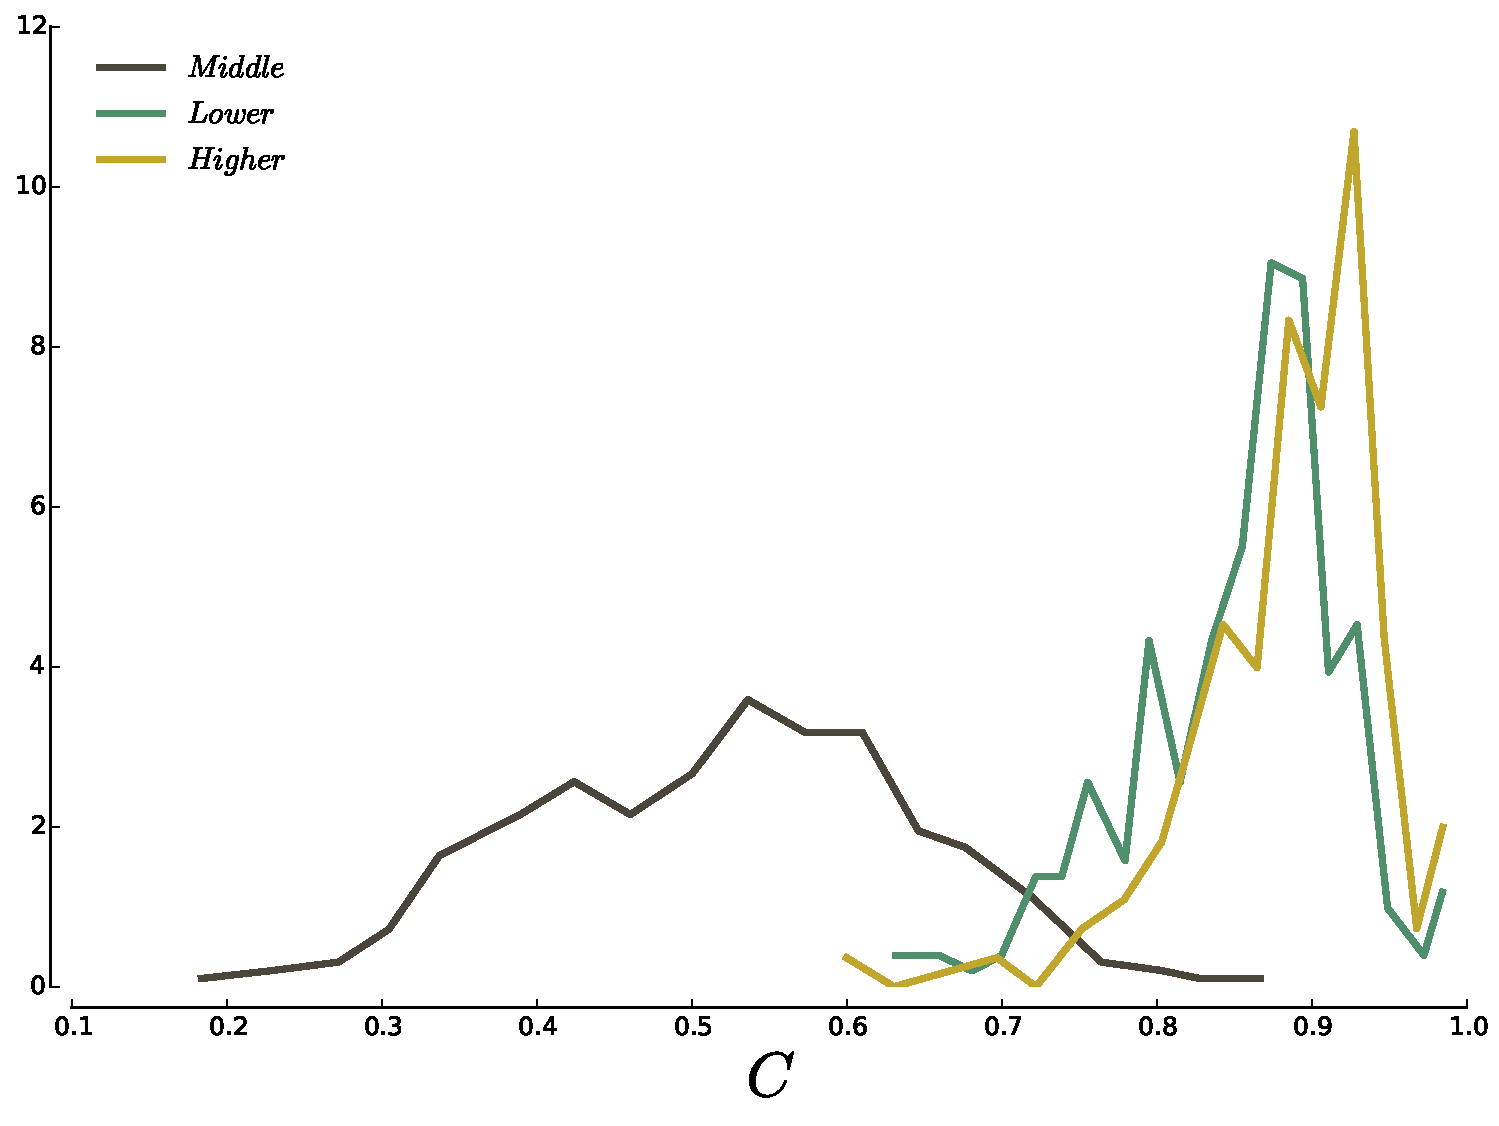
\includegraphics[width=0.7\textwidth]{gfx/chapter-segregation/clustering.pdf}\\
    \caption{{\bf Clustering coefficient.} Distribution of the value of the clustering coefficient for
        all cities in our dataset, for the 3 classes. The higher income class
        exhibits the highest level of clustering, with an average of
        $\overline{C} = 0.90$, followed by the lower income class with on
        average $\overline{C} = 0.87$. The Middle income class households are
        significantly less clustered than the previous two, with $\overline{C} =
        0.56$ on average.} 
        \label{fig:clustering} 
\end{figure}



\subsection{Concentration in neighbourhoods}
\label{sub:concentration_in_neighbourhoods}


If a given class is overrepresented in a neighbourhood, it does not however mean
that most of the individuals belonging to this class live in this neighbourhood.
We compute the ratio of households of each income class that lives in a
neighbourhood over the total number of individuals in the income class (for
rich, poor, and middle class).  Results (Figure~\ref{fig:content}) indicate that
essentially less than $50\%$ of each class live in their respective neighbourhood, while
the rest is dispatched over the rest of the city. The average concentration
decreases from higher-income individuals ($50\%$), to lower-income ($48\%$) and
middle-income individuals ($32\%$).\\

\begin{figure} 
    \centering
    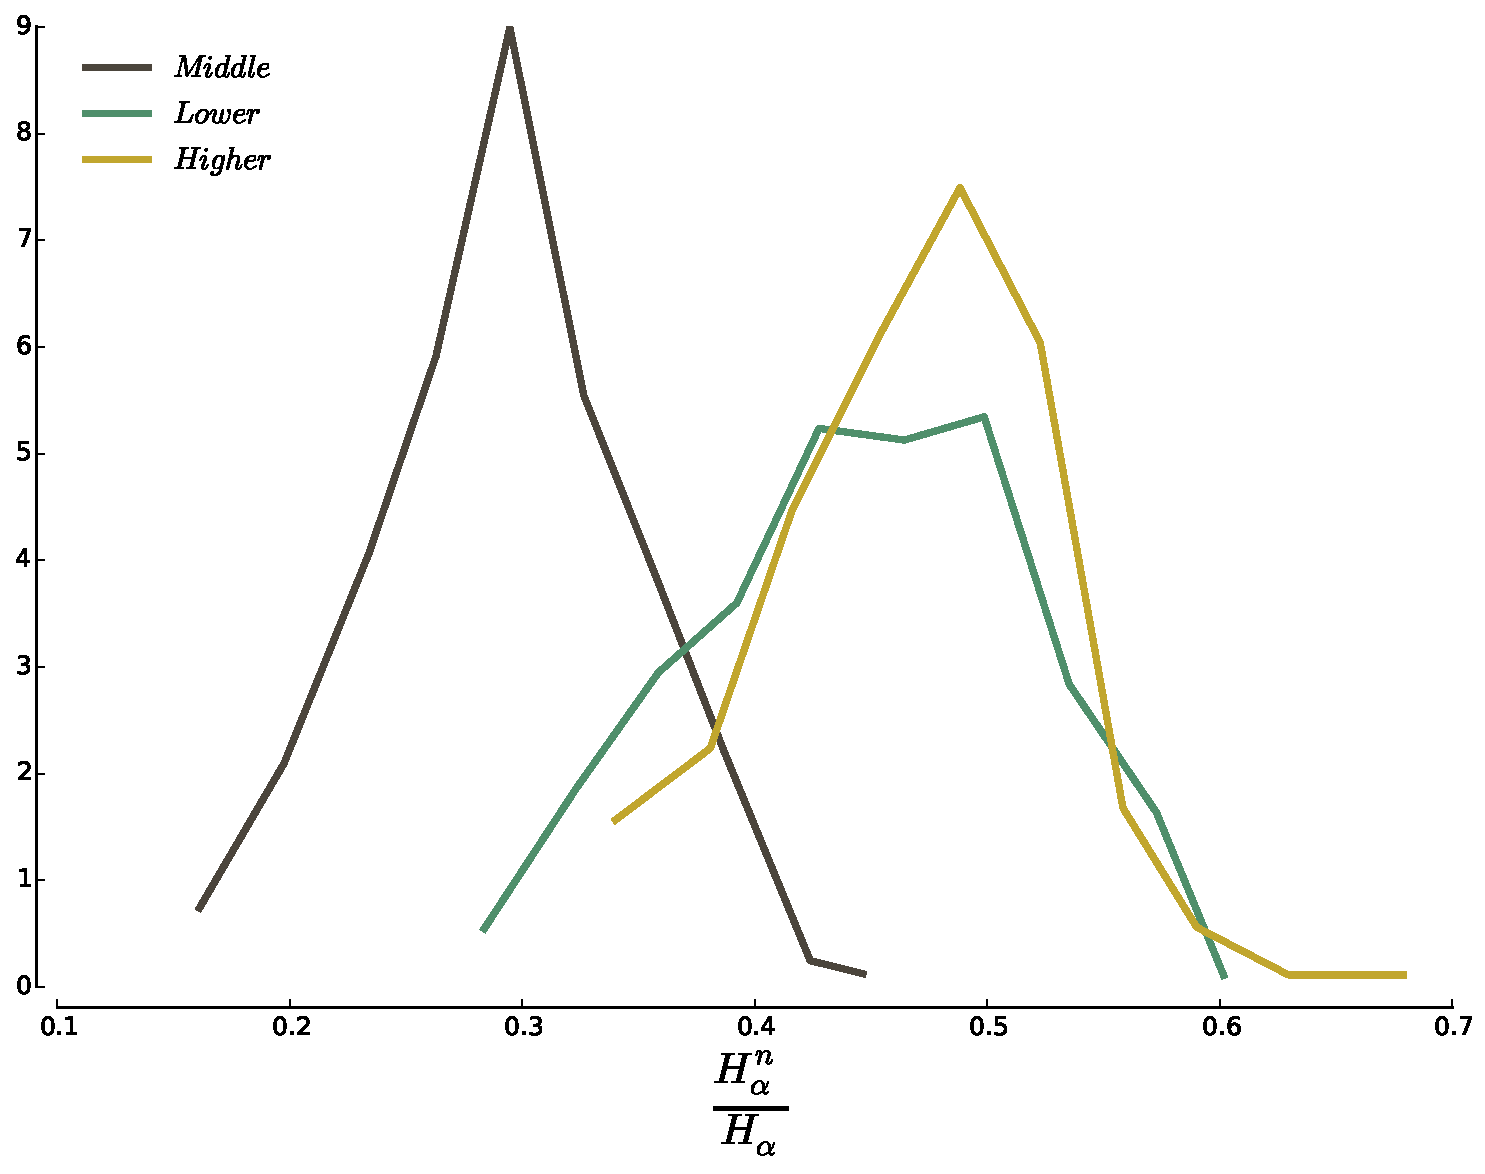
\includegraphics[width=0.7\textwidth]{gfx/chapter-segregation/neighbourhoods_content.pdf}\\
    \caption{{\bf Concentration in neighbourhoods.} Distribution of the fraction of households belonging to a
      given class and that live in a neighbourhood where it is
      overrepresented (Middle, Lower, or Higher).} 
        \label{fig:content} 
\end{figure}



\subsection{One large neighbourhood, or several small ones?}
\label{sub:one_large_neighbourhood_or_several_small_ones_}

Finally, large values of clustering can hide different situations. We
could have on one hand a `giant' neighbourhood and several isolated areal units, which
would essentially mean that each class concentrates in a unique
neighbourhoods. Or on the other hand, several neighbourhoods of
similar sizes, meaning that the different classes concentrate in
several neighbourhoods across the city. In order to distinguish
between the two situations, we plot

\begin{equation} 
    P = H_{2}^N / H_{1}^N 
\end{equation}

where $H_{1}^N$ is the population of the largest neighbourhood, and $H_{2}^N$
the population of the second largest neighbourhood. The results are shown on
Figure~\ref{fig:polycentrism}, and again show a different behaviour for the
middle-income on one side, and higher-income and lower-income on the other side.
The size of the middle-income neighbourhoods are relatively balanced, with on average
$P=0.62$.  Higher- and lower-income neighbourhoods, on the other hand, are
dominated by one big neighbourhood, with respectively $P=0.22$ and
$P=0.26$ on average. 

\begin{figure} 
    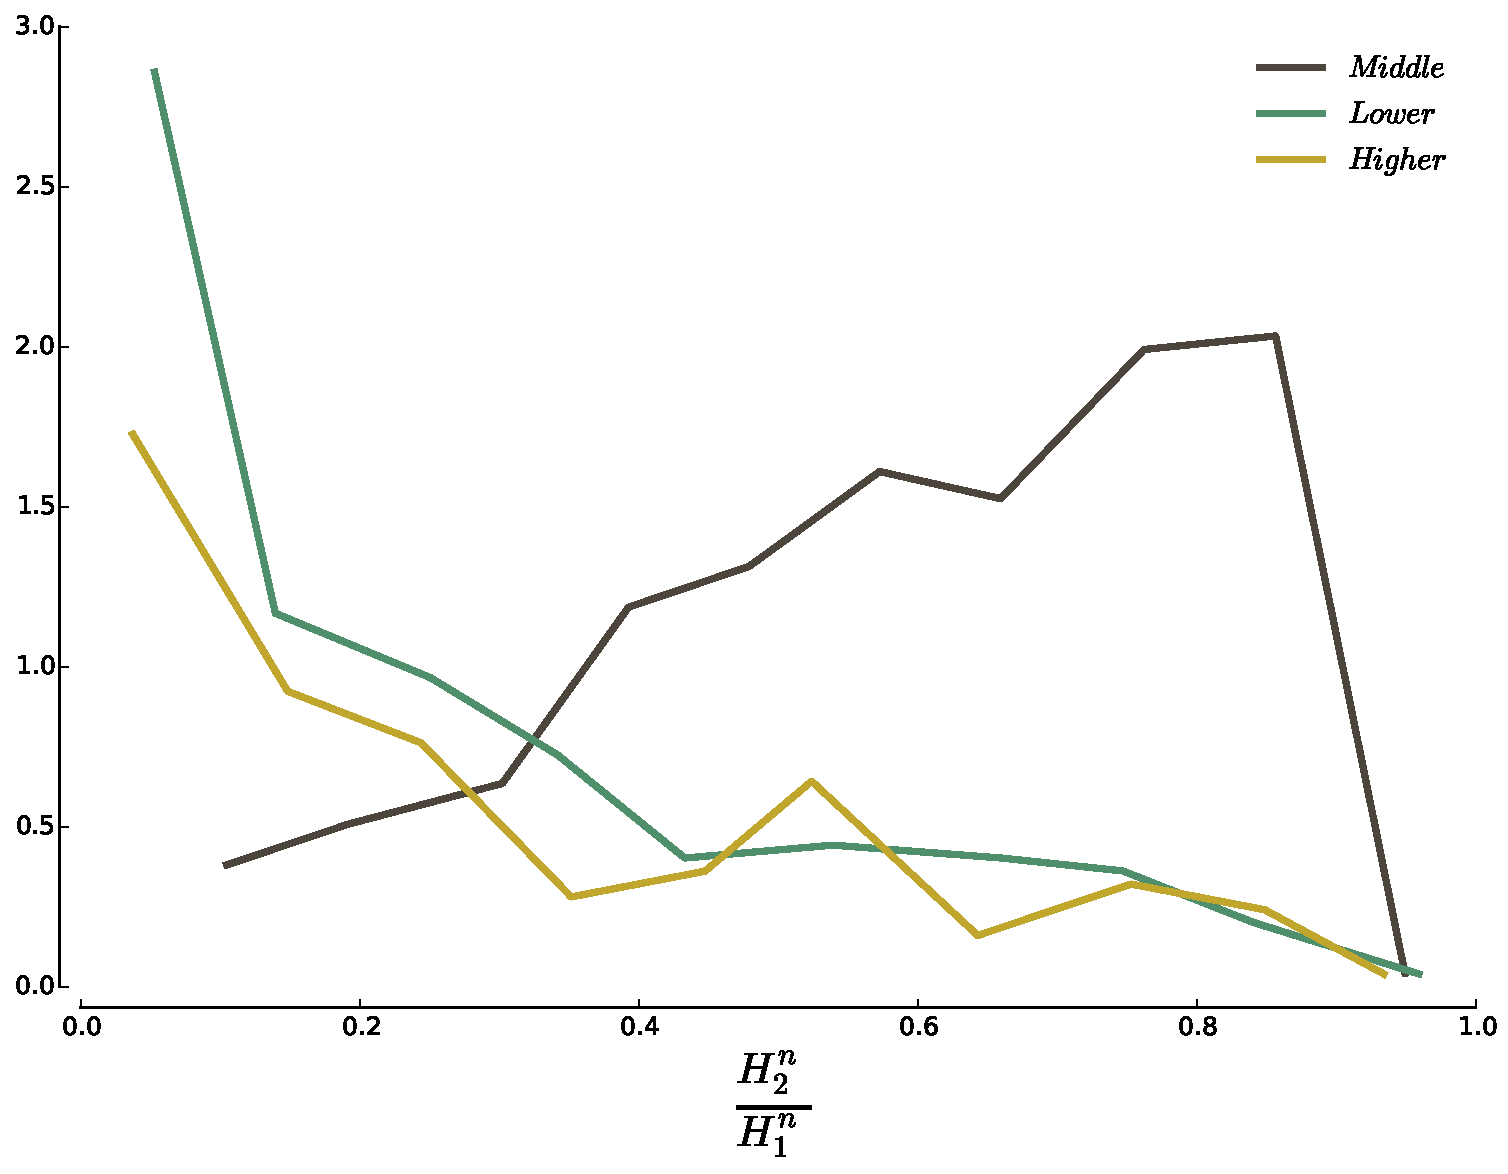
\includegraphics[width=0.7\textwidth]{gfx/chapter-segregation/neighbourhoods_polycentrism.pdf}\\
    \caption{{\bf Poly-neighbourhoods. } Distribution of the ratio of the size of the
        largest and second largest neighbourhoods for each class for all MSA in
        the US. Higher- and lower-income househols tend to concentrate in single
        neighbourhood, with a secondary center that is on average $22\%$ and
        $26\%$ the size of the largest one, respectively. Middle-income
        households tend to be more dispersed, with a secondary neighbourhood that is on
        average $62\%$ of the size of the largest.} 
        \label{fig:polycentrism} 
\end{figure}

 \subsection{Scaling of the number of neighbourhoods}
       \label{ssub:dependence_on_city_size}
       
The clustering values are high, indicating that the neighbourhoods occupied by
households of different classes are very coherent. We can now wonder whether
there is an effect of the city size on the number of neighbourhoods. We plot on
Figure~\ref{fig:number_clusters_class} the number of neighbourhoods found for all
three classes as a function of population. For each class, The curve is
well-fitted by a powerlaw function of the form

\begin{figure}
    \centering
    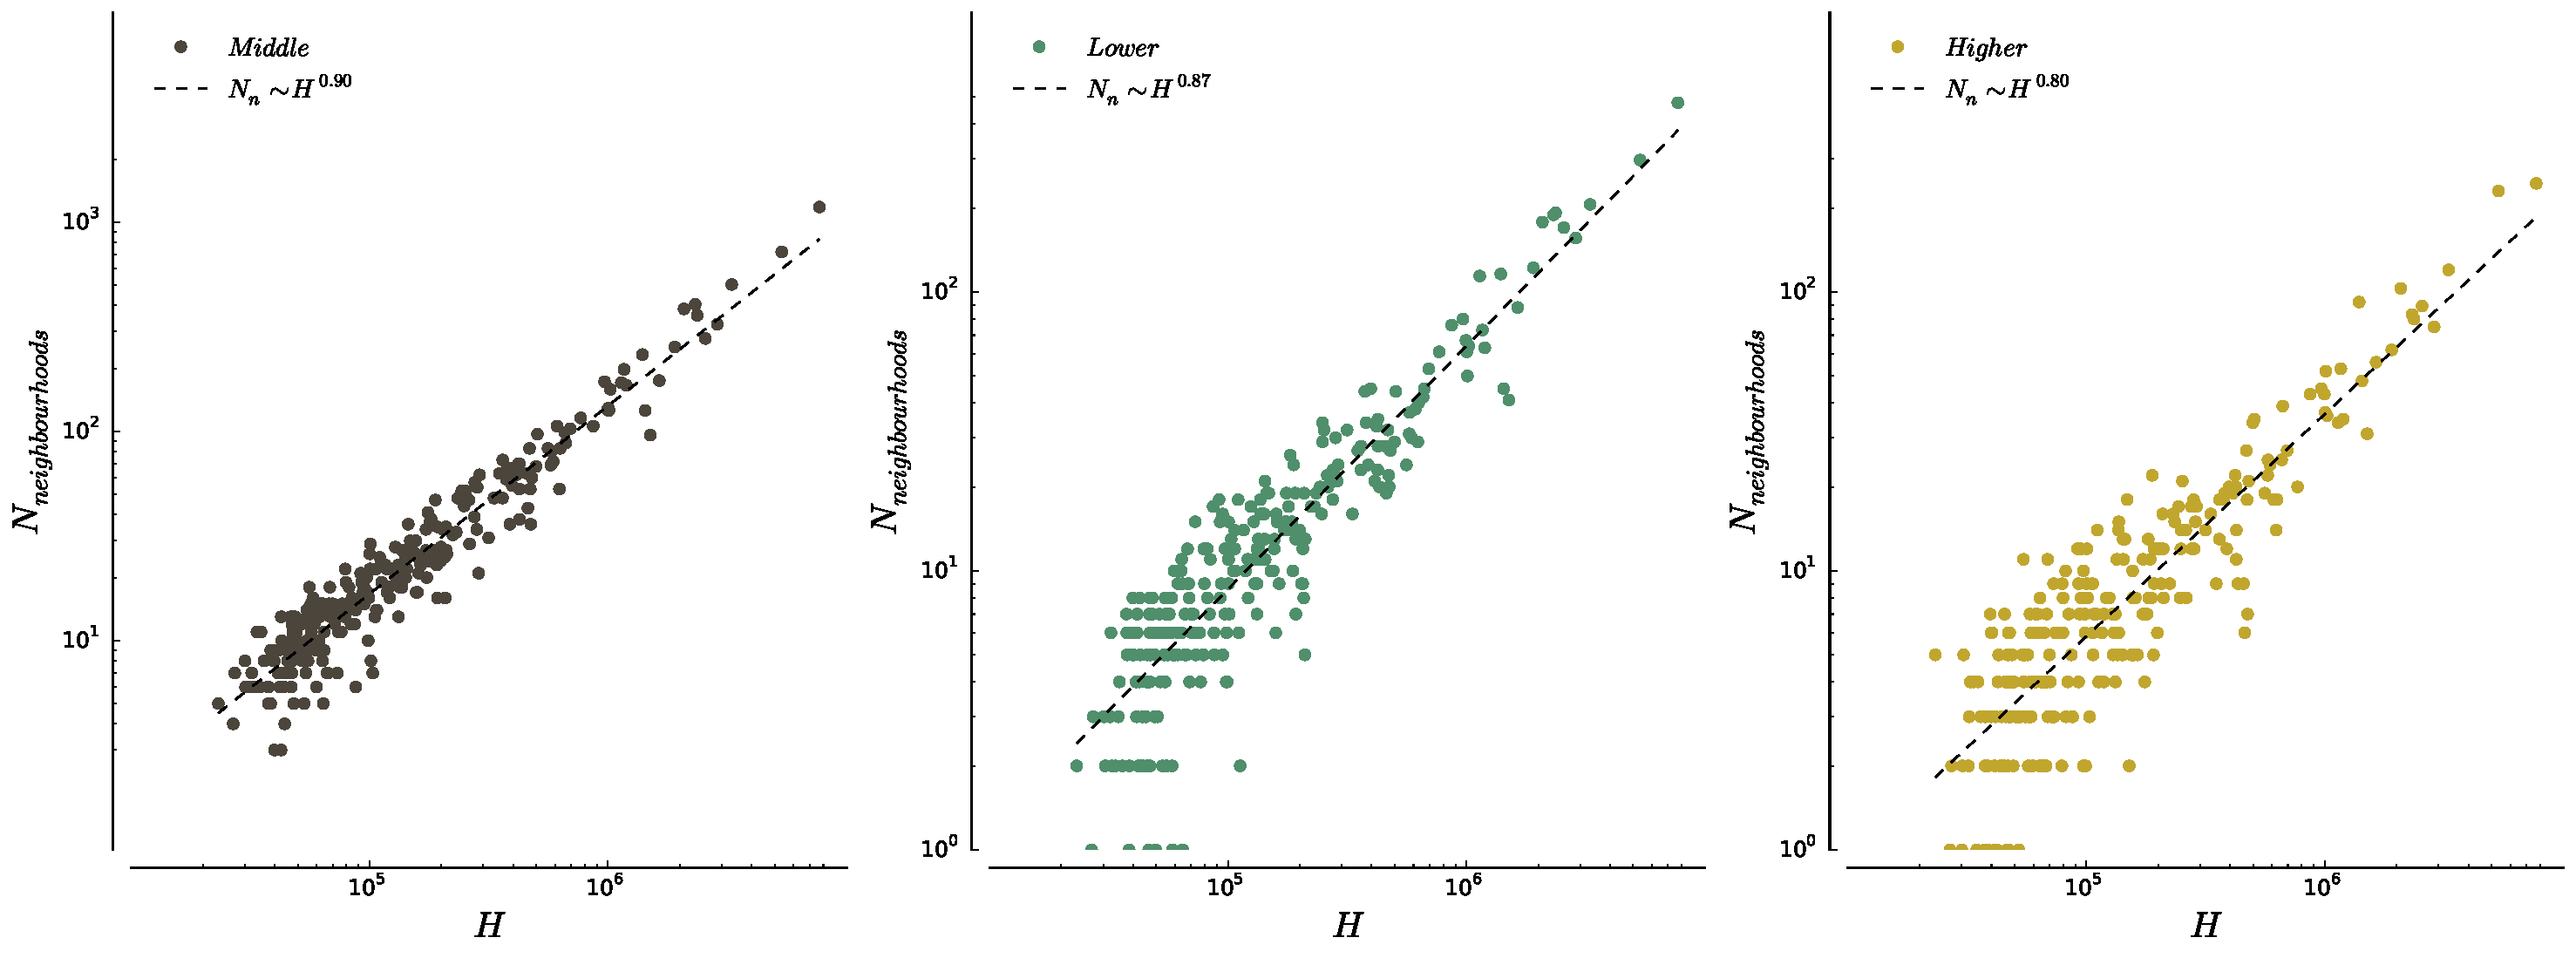
\includegraphics[width=\textwidth]{gfx/chapter-segregation/figure7.pdf}
    \caption{{\bf Number of neighbourhoods and city size.} Number of neighbourhoods for the three different classes as a
    function of the size of the city. These plots in loglog show that
    we have a behavior consistent with a power law with exponent less
    than one (and with different value for each class), with $r^2$ values that
    range between $0.88$ (higher-income) and $0.96$ (middle-income). Combined with the linear
    increase of the number of over-represented units with the number of
    households, this sub-linear increase in the number of neighbourhoods shows the tendency of
classes to cluster more as cities get larger.\label{fig:number_clusters_class}}
\end{figure}

\begin{equation}
    N_n = b\,H^\beta
\end{equation}

where the exponent $\beta$ is less than one and depends on the class, 
indicating that there are proportionally less neighbourhoods
in larger cities (the number areal units scales proportionally with the
population size). The values of the exponents are

\begin{align*}
    \beta_{H} = 0.80\\
    \beta_{L} = 0.87\\
    \beta_{M} = 0.90\\
\end{align*}

One is tempted to conclude from these numbers that the different classes
become more spatially coherent as the population increases. 
Yet, this conclusion only holds if the number of areal units in which each class
is overrepresented does not itself vary sublinearly with population size. We
plot on Figure~\ref{fig:overrepresented} these numbers as a
function of the size of the city. We find that the behaviour of the number of
overrepresented units is consistent with a linear behaviour for all three
classes. Together with the exponents above, this shows that the tendency
of the classes to cluster is greater as the city size increases.

In other words, the different classes are more spatially isolated as the city
size increases, implying higher levels of spatial segregation. We note that the
phenonemenon is more important for higher-income households than for lower- and
middle-income households, justifying to an extent the existence of the
expression `ghettos for the rich'.\\

\begin{figure}
    \centering
    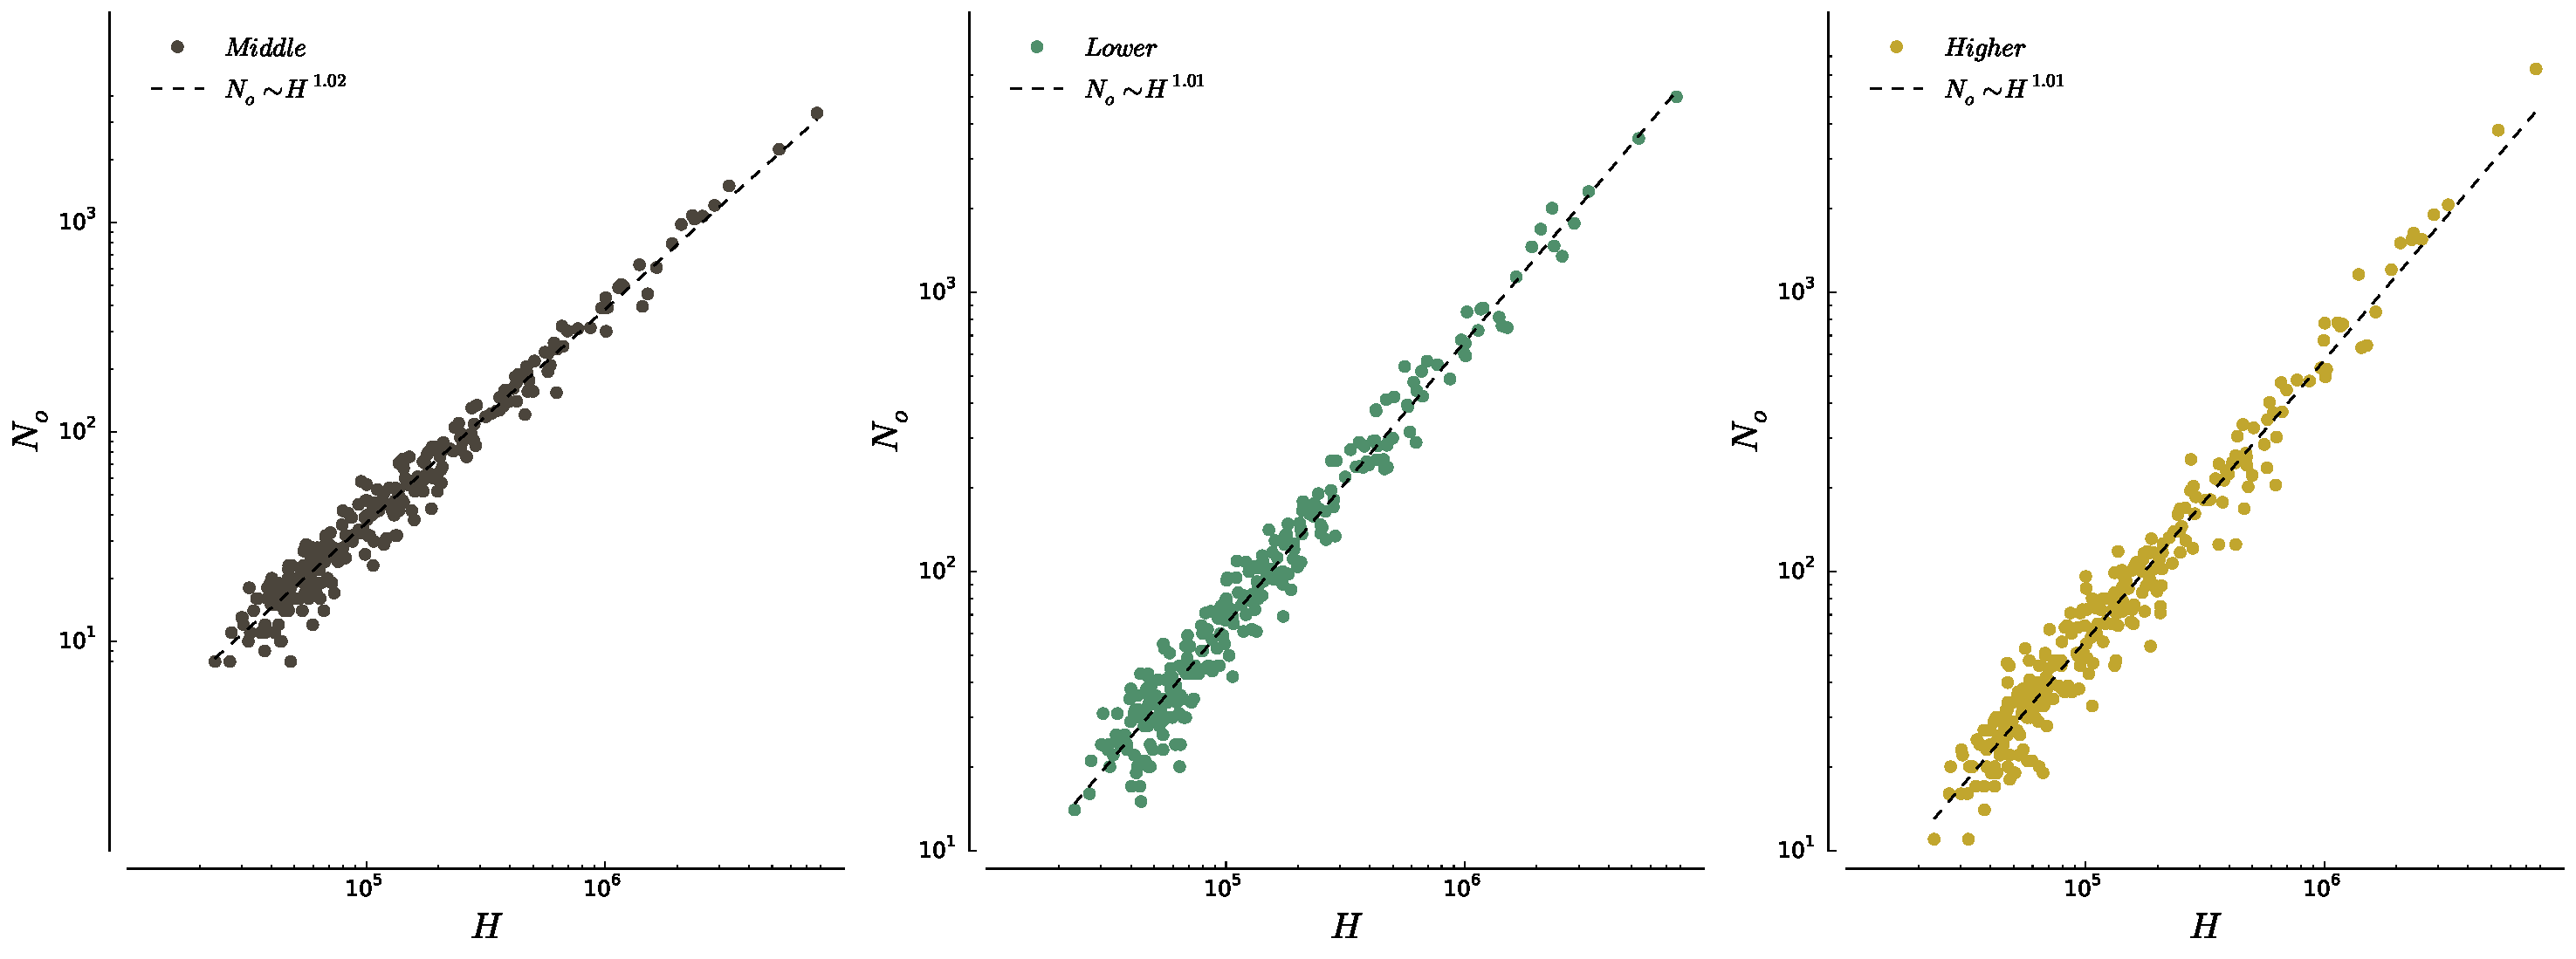
\includegraphics[width=\textwidth]{./gfx/chapter-segregation/number_overrepresented.pdf}
    \caption{{\bf Number of overrepresented areal units and city size.} Number of areal units where each class is overrepresented as a
    function of the total number of households in the city. The behaviour is
consistent with a linear behaviour in the three cases.
\label{fig:overrepresented}}
\end{figure}


\section{Poor centers, rich suburbs?}
\label{sec:poor_centers_rich_suburbs_}

In many studies, the question of the spatial pattern of segregation is limited
to the study of the center versus suburb and is usually adressed in two
different ways. First, a central area is defined by arbitrary boundaries and
measures are performed at the scale of the so-called center and at the scale of
the  rest, labelled as `suburbs'. The issue with this approach is that the
conclusions depend on the chosen boundaries and there is no unique unambiguous
definition of the city center: while some consider it to be the Central Business
District~\cite{Glaeser:2008}, others choose to define the center as the urban
core (urbanized area), where the population density is higher. The second
approach, in an attempt to get rid of arbitrary boundaries, consists in plotting
indicators of wealth as a function of distance to the
center~\cite{Glaeser:2008}. This approach, inspired by the monocentric and
isotropic city of many economic studies such as the Von Th\"unen or the
Alonso-Muth-Mills model~\cite{Brueckner:1987}, has however a serious flaw:
cities are not isotropic and are spread unevenly in space, leading to very
irregular shapes~\cite{Makse:1995}. Representing any quantity versus the
distance to a center thus amounts to average over very different areas and is necessarily misleading in
clear polycentric cases (as it is the case for large cities
~\cite{Louf:2013_polycentric}. See also
Chapter~\ref{chap:monocentric_introduction}). The notion of distance to the center is indeed
meaningless in polycentric situations.\\


We propose here a different approach that does not require the
definition of a distance to the center. Instead, we plot the average
representation computed over all areal units (Census blockgroups in this
dataset) with a given density population $\rho$, as a function of the density
$\rho$. Indeed, what is usually meant by `center' of a city are the areas with
the highest residential (or employment) densities. 

Our findings shed a new light on the difference of social composition
between the high-density and low-density areas in cities. As shown on
Figure~\ref{fig:high_low_densities}, we find that rich households are
overrepresented in low-density regions on average. While this agrees well with
the opinion people have of suburbian America, there is a more surprising result:
higher income households are also overrepresented in areas with very large densities
(typically above $20,000$ inhabitant$/\text{km}^2$). In between, neighborhoud
with intermediate values of density (between $1,000$ and $20,000$
inhabitants$/\text{km}^2$), are lower-income neighbourhoods. 

Only few cities in the US have neighbourhoods that reach the threshold of
$20,000$ inhabitants per km$^2$, which can explain why we observe in most cases
poor centers and rich suburbs. We can wonder whether the difference usually
discussed between North American and European cities does not come, in fact,
from differences in terms of densities. 

\begin{figure}
    \centering
    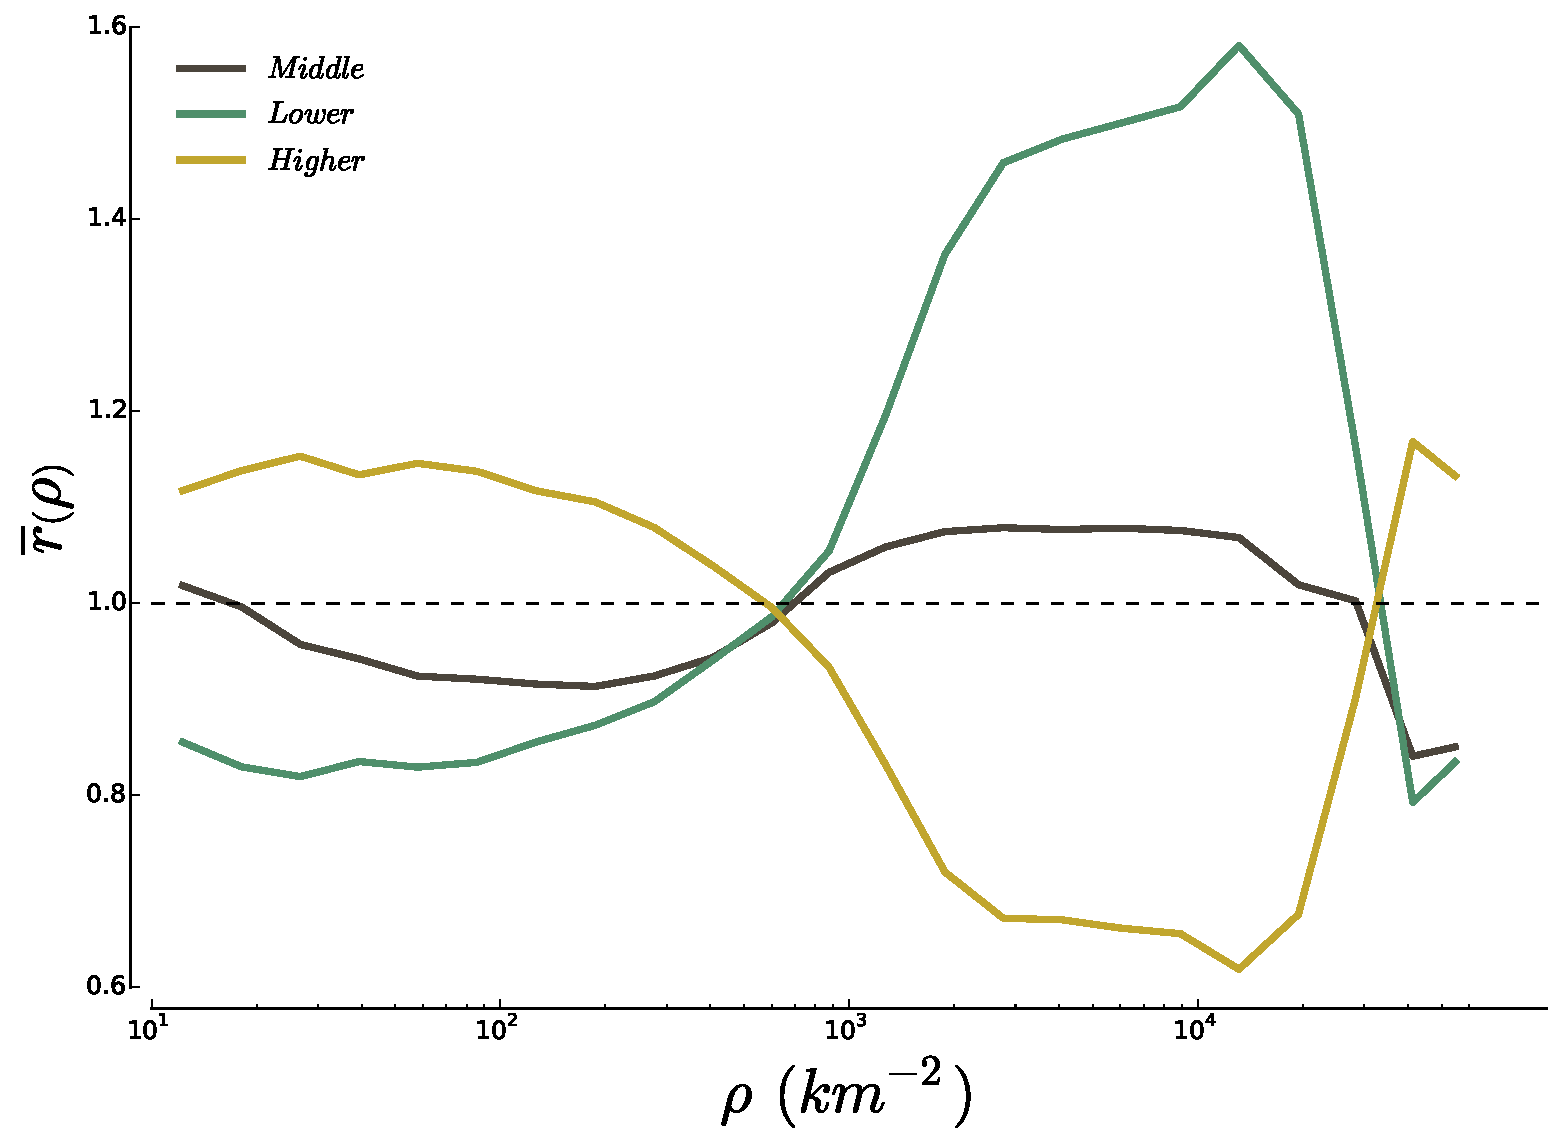
\includegraphics[width=\textwidth]{gfx/chapter-segregation/figure4.pdf}
    \caption{{\bf Representation and density.} Average representation of the higher-, middle- and
      lower-income classes over the $276$ MSA as a function of the
      local density of households. On average, we find that low-density regions (the
      suburbs) are rich, while high density regions (the center) are poor,
      confirming empirically on a large dataset a stylized facts that had previously
      emerged from local studies. Interestingly, we also
      find that  very large density areas ($\rho>20,000/km^2$) are rich on average,
      suggesting that density may be one relevant element in an eventual
      explanation of the differences between neighbourhoods~\cite{Jacobs:1961}.
      \label{fig:high_low_densities}
  } 
  \end{figure}

\section{Conclusion and perspective}
\label{sec:conclusion_and_perspective}

Instead of attempting to define segregation by enumerating its different
aspects, we took a radically different -- yet simpler -- approach. We chose to
define segregation through specifying what it is not.  This naturally lead to
defining the measure of representation, which is used in turn to delineate
neighbourhoods. We further defined the exposure (still based on the
representation), which measures the extent to which different categories
attract, repel or are indifferent to one another.

We then showed that we can define classes in a non-parametric way and 3 main
income classes emerged for the 2000 US Census data. The middle-income class
corresponds to a smaller income range than what is usually admitted, a curiosity
that certainly deserves further investigations. In terms of spatial arrangement,
although the fraction of the population that is contained in neighbourhoods does
not change with city size, the neighbourhoods are geographically more coherent
as cities get larger, which corresponds in effect to an increased level of
segregation as the size of the city increases. The behaviors of different
categories are very coherent and we showed that we could simplify the
description of these complex systems by reducing the sometimes large number of
categories to a small number of classes. This is an important point which will
simplify the description and modeling of stratification mechanisms.

Our results point to the intriguing fact that higher-income households are on
average overrepresented in very dense areas. Such high density areas are
relatively rare in the US, which might explain in part why authors have
traditionally simplified the picture, talking about poor
centers and rich suburbs. This result echoes Jane Jacobs' analysis~\cite{Jacobs:1961}
that neighbourhoods with the highest dwelling densities usually are the ones
exhibiting the most vitality, and therefore the most attractive. Of course, high
densities are not everything, and some high-density neighbourhoods also are
lower-income neighbourhoods. Further investigations along these lines may
provide quantitative insights into the mechanisms leading to urban decline or
urban regeneration.\\

In this Chapter, we have tried to highlight the \emph{spatial} pattern of
segregation.  We believe that the identification of neighbourhoods that our
method permits will allow a finer-scale investigation of these spatial patterns.
The fundamental issue that runs beneath, however,  is the need for a useful,
simplified description of spatial density. A problem yet to be solved, but that
has a huge potential of applications. We note that the problem is tightly
linked, if not identical, to the one we encountered while trying to describe the
spatial distribution of density in Chapter~\ref{chap:monocentric_discussion}.
